\documentclass[letterpaper]{article}
\usepackage{aaai}
\usepackage{algorithm}
\usepackage[noend]{algpseudocode}
\usepackage[numbers]{natbib}
\bibliographystyle{plainnat}

\makeatletter
\def\BState{\State\hskip-\ALG@thistlm}
\makeatother

\usepackage{hyperref}
\usepackage{amsmath}
\usepackage{lmodern}
\usepackage{courier}
\usepackage{listings}
\usepackage{graphicx}
\usepackage{tabularx}
\usepackage{tikz}
\usetikzlibrary{bayesnet}
\usetikzlibrary{arrows}
\graphicspath{ {figures/} }

\lstset{basicstyle=\ttfamily\footnotesize,breaklines=true}

\setlength{\pdfpagewidth}{8.5in}
\setlength{\pdfpageheight}{11in}
\pdfinfo{
  /Title (Topic Modeling for Scientific Documents)
  /Author (Jethro Kuan)}
\begin{document}
\nocopyright

\title{Topic Modeling for Scientific Documents}
\author{Jethro Kuan \\
  WING-NUS\\
}
\maketitle
\begin{abstract}
  \begin{quote}
    Topic modeling is a statistical modeling technique used to
    discover abstract topics that occur in a collection of documents.
    Topic modeling can be applied to scientific documents for data
    discovery and navigation, among others. In this paper, we discuss
    the predominant technique for topic modeling, the Latent Dirichlet
    Allocation, and its extensions. We show how to train these models,
    by providing a walk-through with a dataset of scientific
    documents. We discuss the differences between the topic models,
    and elaborate on their strengths and shortcomings.
  \end{quote}
\end{abstract}

\section{Introduction}
In this information age, the availability of knowledge is
insufficiently met with the tools to navigate it. Archives such as
Arxiv see an exponential growth in the number of documents being
hosted. Developing new tools for browsing, and searching these
documents is a technological challenge that calls for research in
statistical modeling.

Rather than relying on keyword matching, tools like Semantic Scholar
use machine learning to process scientific documents and discover
meaningful structure, empowering researchers to discover papers more
relevant to their work. One such statistical modeling technique is
topic modeling.

Topic modeling attempts to discover abstract topics within documents.
Topic models capture the intuition that if a document is of a
particular topic, then words from the topic should appear more
frequently.

A topic model trained on a corpora of scientific documents could learn
topics such as ``Neural Networks'', ``Biology'' and ``Medicine''.
Topics attribute a high probability to words that relate to the topic.
For example, a ``Neural Networks'' topic would give attribute a high
probability to ``classifiers'', and a low probability to ``bacteria''.
The quotations around the topics are to make explicit that the labels
are human interpretations of what these topics may be. Topic modeling
is an unsupervised problem, and is often trained on unlabeled data.
Automatic labeling of these topics is an active area of research
\cite{mei2007automatic, lau2011automatic}.

We can also view these abstract topics as a form of clustering.
Researchers are better able to navigate the large corpora of
scientific knowledge, by looking at documents that have similar topic
proportions\footnote{A browsable 100-topic model estimated from the
  Journal \textit{Science} can be explored at
  \url{http://www.cs.cmu.edu/~lemur/science/topics.html}}.

\begin{figure}[ht]
  \centering
  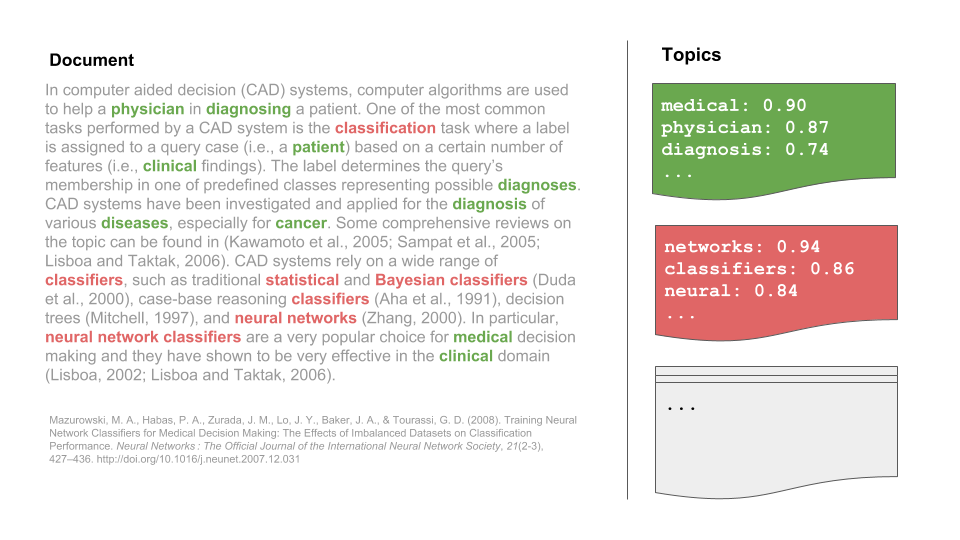
\includegraphics[width=0.5\textwidth]{topic_models.png}
  \caption{\label{fig:topic_model_document} According to the trained
    topic model, topics like ``Medicine'' and ``Neural Networks''
    generate the colored words of the document}
\end{figure}

Suppose we train a topic model on a corpora of scientific documents.
The trained model would discover that the document in
~\autoref{fig:topic_model_document} relates to ``Medicine'' and
``Neural Networks'', because of the frequent appearance of highly
probable words in these topics.

The earliest known technique for topic modeling is Latent Semantic
Indexing (LSI) \cite{deerwester1990indexing}. LSI uses Singular Value
Decomposition (SVD) to determine relationships between words in
unstructured text. The first probabilistic approach, Probabilistic
Latent Semantic Analysis (pLSA), was proposed in 1999
\cite{hofmann1999probabilistic}. It was only in 2003 when
\citeauthor{blei2003latent} introduced Latent Dirichlet Allocation
(LDA), which remains the predominant technique for topic
modeling to date.

Most of the state-of-the-art topic models are generative models. In
generative models, latent variables govern the generative process of a
document. A document is produced from a distribution of topics, and
the topics are distributions over the vocabulary of the corpora.

In this paper, we survey the landscape of probabilistic topic models.
LDA and two of its variants are discussed in detail. We train these
models on a dataset of scientific documents, and present our results.

\section{LDA}
Latent Dirichlet Allocation is widely considered to be the simplest
topic model. LDA models each document as a mixture of $K$ topics,
where a topic $\beta_k$ is a probability distribution over a fixed
vocabulary of terms. LDA is a directed graphical model, and can be
represented in plate notation like in ~\autoref{fig:lda_plate}.

At the risk of being pedantic, we explain the components of the
graphical model. $\eta$ is the topic hyperparameter, which produces a
topic distribution $\beta_k$ of the Dirichlet family. There are a
total of $K$ topics. $\alpha$ is a hyperparameter that
produces the per-document topic proportions $\theta_d$. These
Dirichlet distributions are of dimension $K-1$, because there are a
total of $K$ topics. There are $D$ such topic proportions, where $D$
is the total number of documents. $Z_{d,n}$ is the per-word topic
assignment, drawn from the particular $\theta_d$. Finally, $W_{d,n}$
is the $n$th word in the $d$th document, an observed variable. It is
simple to see that
$P(W_{d,n} | Z_{d,n}, \beta_{k}) = \beta_{z_{d,n}, w_{d,n}}$.

A high $\alpha$ value encodes the belief that documents contain a
mixture of many topics, rather than being largely represented by a few
topics. Similarly, a high $\eta$ value encodes the belief that topics
has high probability for a large number of words in the vocabulary.

\begin{figure}[ht]
  \centering
  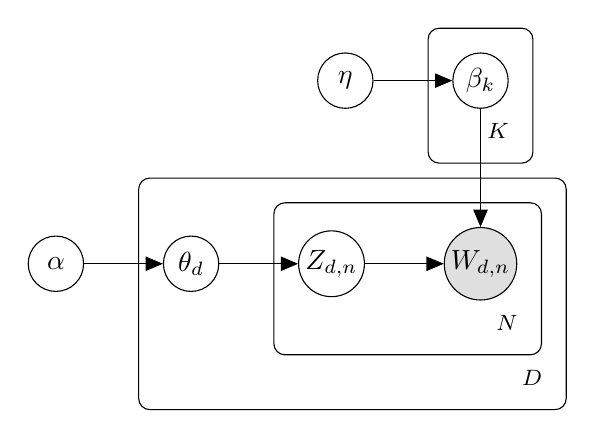
\begin{tikzpicture}
    \node[latent] (a) {$\alpha$};
    \node[latent, right=of a] (t) {$\theta_d$};
    \node[latent, right=of t] (z) {$Z_{d,n}$};
    \node[obs, right=of z] (w) {$W_{d,n}$};
    \node[latent, above=1.5cm of w] (b) {$\beta_k$};
    \node[latent, left=of b] (e) {$\eta$};

    % Edges
    \edge {a} {t};
    \edge {t} {z};
    \edge {z} {w};
    \edge {e} {b};
    \edge {b} {w};

    % Plates
    \plate [inner sep=0.3cm] {pN} {(z)(w)} {$N$};
    \plate [inner sep=0.3cm] {pM} {(t)(z)(w)(pN)} {$D$};
    \plate [inner sep=0.3cm] {pK} {(b)} {$K$};
  \end{tikzpicture}
  \caption{\label{fig:lda_plate} Plate notation for LDA.}
\end{figure}

The model is fully specified by its joint distribution $\mathcal{J}$
of all the latent and observed variables.

\begin{multline}
 \mathcal{J} = \left( \sum_{k=1}^{K} P(\beta_k | \eta) \right) \left(
    \sum_{d=1}^{D} P(\theta_d | \alpha) \right) \\
  \left( \sum_{n=1}^{N} \theta_{d, Z_{d,n}} \beta_{Z_{d,n}, W_{d,n}} \right)  
\end{multline}

The generative process of a document is as follows:

\begin{algorithm}
  \caption{Generative Process of LDA}\label{alg:LDA}
  \begin{algorithmic}[1]
    \For {each document $d$ in $D$}
    \State {Draw topic distribution $\theta_d \sim Dir(\alpha)$}
    \For {each word $n_d$ in $N_d$}
    \State {Sample topic $z_{d,n} \sim Multinomial(\theta)$}
    \State {Sample word $w_{d,n} \sim Multinomial(\beta_{z_{d,n}})$}
    \EndFor
    \EndFor
  \end{algorithmic}
\end{algorithm}

If we fix the topic distributions $\beta_{1:K}$, we can compute the
per-document posterior $\theta$ given the document.

\begin{multline}
  P(\theta | w_{1:n}, \alpha, \beta_{1:K}) = \\ \frac{P(\theta |
    \alpha)\prod_{n=1}^{N} P(z_n | \theta) P(w_n | z_n,
    \beta_{1:K})}{\int_\theta P(\theta | \alpha) \prod_{n=1}^N
    \sum_{z=1}^K P(z_n | \theta) P(w_n | z_n, \beta_{1:K})}
\end{multline}

The denominator is intractable to compute, due to the coupling
between $\theta$ and $\beta$ under the multinomial assumption.
\cite{blei2003latent}. Hence, we rely on techniques for approximate
inference of the posterior. We discuss these techniques in
~\autoref{sec:inference}.

Why does LDA work? The Dirichlet distribution encourages sparsity,
encoding the belief that the document-topic distribution has few
topics per document, and the topic-word distribution has few words per
topic. These two beliefs work against each other, and LDA discovers
this sparsity balance, which gives rise to the structure of the
textual data.

\subsection{Statistical Assumptions}
\label{subsec:statistical-assumptions}
In Bayesian statistics, we cannot make inference without statistical
assumptions. LDA makes several statistical assumptions, which we
discuss below.

First, LDA models documents as ``bag-of-words''. In a ``bag-of-words''
model, words within the document are exchangeable
\cite{blei2003latent}. I think this is a reasonable assumption to
make, if the task is to discover themes within the document.

Second, LDA assumes that the order of documents does not matter.
Exchangeability of both words and documents allows LDA to model the
joint distribution as a mixture model. I believe this assumption to be
invalid in the domain of scientific documents. The meaning of
keyphrases used in scientific literature change over time. For
example, the landscape of research neural networks is vastly different
now, as compared to the 1990s, and LDA will fail to capture these
differences. This is the motivation of the Dynamic Topic Model (DTM),
discussed in ~\autoref{sec:dtm}.

Third, the use of the Dirichlet distribution also encodes statistical
assumptions about the correlation between topics. Under the Dirichlet,
components of $\theta_d$ are nearly independent. This leads to the
modeling assumption that the presence of one topic is not correlated
with the presence of another \cite{blei2005correlated}. As explained
by \citeauthor{blei2005correlated}, this assumption is strong and
unrealistic in the domain of scientific documents. An article about
genetics is also highly likely to be about health and disease, and
unlikely to be about astronomy. This is the motivation of the
Correlated Topic Model (CTM), which we discuss next.

\section{Correlated Topic Modeling}
\label{sec:ctm}
The Correlated Topic Model (CTM) addresses the model assumption that
topic proportions are not correlated.

Instead of drawing from a Dirichlet distribution, the CTM uses a
logistic normal distribution. CTM draws a real valued random vector
from a multivariate Gaussian, and maps it to the simplex to obtain a
multinomial parameter \cite{blei2005correlated}. The $K \times K$
covariance matrix $\Sigma$ models correlations between the topics.
This tweak is evident in the generative process shown in Algorithm
~\autoref{alg:CTM}, contrasting it with Algorithm ~\autoref{alg:LDA}.

\begin{algorithm}
  \caption{Generative Process of CTM}\label{alg:CTM}
  \begin{algorithmic}[1]
    \For {each document $d$ in $D$}
    \State {Draw topic distribution $\beta_d \sim \mathcal{N}(\mu, \Sigma)$}
    \For {each word $n_d$ in $N_d$}
    \State {Sample topic $z_{d,n} \sim Multinomial(\pi(\beta_d))$}
    \State {Sample word $w_{d,n} \sim Multinomial(\beta_{z_{d,n}})$}
    \EndFor
    \EndFor
  \end{algorithmic}
\end{algorithm}

$\pi$ maps the multinomial parameters to the mean parameters,
$\pi\left( x \right) = \frac{e^x}{\sum_{i} e^{x_i}}$

\begin{figure}[ht]
  \centering
  \begin{tikzpicture}
    \node[latent] (S) {$\Sigma$};
    \node[latent, left= of t, yshift=-1cm] (m) {$\mu$};
    \node[latent, right= of S, yshift=-0.5cm] (t) {$\theta_d$};
    \node[latent, right=of t] (z) {$Z_{d,n}$};
    \node[obs, right=of z] (w) {$W_{d,n}$};
    \node[latent, above=1.5cm of w] (b) {$\beta_k$};
    \node[latent, left=of b] (e) {$\eta$};

    % Edges
    \edge {S} {t};
    \edge {m} {t};
    \edge {t} {z};
    \edge {z} {w};
    \edge {e} {b};
    \edge {b} {w};

    % Plates
    \plate [inner sep=0.3cm] {pN} {(z)(w)} {$N$};
    \plate [inner sep=0.3cm] {pM} {(t)(z)(w)(pN)} {$D$};
    \plate [inner sep=0.3cm] {pK} {(b)} {$K$};
  \end{tikzpicture}
  \caption{\label{fig:ctm_plate} Plate notation for CTM.}
\end{figure}


The Multinomial and Gaussian distributions are not conjugate
distributions. This causes difficulty in inference via Gibbs sampling,
and variational inference is used instead.

\section{Dynamic Topic Modeling}
\label{sec:dtm}
Dynamic Topic Modeling (DTM) was proposed to remove the assumption
that documents are \textit{exchangeable}. \cite{blei2006dynamic}

The order of documents is important for scientific documents, since
both the content, and the meaning of words evolve over time.

In DTM, data is divided by discrete time slices. The topics associated
with time slice $t$ evolve from the time slice $t-1$. Because the
Dirichlet distribution is not amenable to sequential modeling, we use
the Gaussian distribution to model the sequence of random variables.

The generative process for time slice $t$ is as follows:

\begin{algorithm}
  \caption{Generative Process of DTM}\label{alg:DTM}
  \begin{algorithmic}[1]
    \State {Draw topic distribution $\beta_t | \beta_{t-1} \sim N(\beta_{t-1},
  \sigma^2I)$}
    \State {Draw $\alpha_t | \alpha_{t-1} \sim N\left( \alpha_{t-1}, \delta^2I
    \right)$}
    \For {each document $w$}
    \State {Draw $\eta_{w,t} \sim N\left( \alpha_t, a^2I \right)$}
    \For {each word at position $n$}
    \State {Sample topic $z_{t,n} \sim Multinomial(\pi(\eta_{w,t}))$}
    \State {Sample word $w_{t,d,n} \sim Multinomial(\beta_{t,z,n})$}
    \EndFor
    \EndFor
  \end{algorithmic}
\end{algorithm}

\begin{figure}[ht]
  \centering
  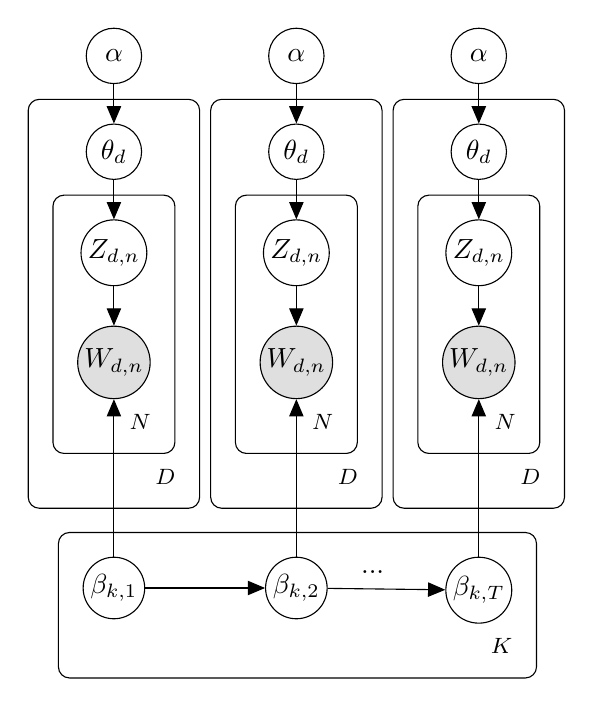
\begin{tikzpicture}
    \node[latent] (a1) {$\alpha$};
    \node[latent, below=0.5cm of a1] (t1) {$\theta_d$};
    \node[latent, below=0.5cm of t1] (z1) {$Z_{d,n}$};
    \node[obs, below=0.5cm of z1] (w1) {$W_{d,n}$};
    \node[latent, below=2cm of w1] (b1) {$\beta_{k,1}$};

    \node[latent, right=1.6cm of a1] (a2) {$\alpha$};
    \node[latent, below=0.5cm of a2] (t2) {$\theta_d$};
    \node[latent, below=0.5cm of t2] (z2) {$Z_{d,n}$};
    \node[obs, below=0.5cm of z2] (w2) {$W_{d,n}$};
    \node[latent, below=2cm of w2] (b2) {$\beta_{k,2}$};

    \node[latent, right=1.6cm of a2] (at) {$\alpha$};
    \node[latent, below=0.5cm of at] (tt) {$\theta_d$};
    \node[latent, below=0.5cm of tt] (zt) {$Z_{d,n}$};
    \node[obs, below=0.5cm of zt] (wt) {$W_{d,n}$};
    \node[latent, below=2cm of wt] (bt) {$\beta_{k,T}$};

    % Edges
    \edge {a1} {t1};
    \edge {t1} {z1};
    \edge {z1} {w1};
    \edge {b1} {w1};

    \edge {a2} {t2};
    \edge {t2} {z2};
    \edge {z2} {w2};
    \edge {b2} {w2};

    \edge {at} {tt};
    \edge {tt} {zt};
    \edge {zt} {wt};
    \edge {bt} {wt};

    \edge {b1} {b2};
    \edge {b2} {bt};
    \node[text=, right=0.3cm of b2, yshift=0.2cm] {...};

    % Plates
    \plate [inner sep=0.3cm] {pN1} {(z1)(w1)} {$N$};
    \plate [inner sep=0.3cm] {pM1} {(t1)(z1)(w1)(pN1)} {$D$};

    \plate [inner sep=0.3cm] {pN2} {(z2)(w2)} {$N$};
    \plate [inner sep=0.3cm] {pM2} {(t2)(z2)(w2)(pN2)} {$D$};

    \plate [inner sep=0.3cm] {pNt} {(zt)(wt)} {$N$};
    \plate [inner sep=0.3cm] {pMt} {(tt)(zt)(wt)(pNt)} {$D$};
    
    \plate [inner sep=0.3cm] {pK} {(b1)(b2)(bt)} {$K$};
  \end{tikzpicture}
  \caption{\label{fig:dtm_plate} Plate notation for DTM.}
\end{figure}

Similar to CTM, the use of the logistic normal distribution causes
variational inference to be the preferred approximate inference
technique.

Further extensions of this approach include the continuous Dynamic
Topic Models (cDTM), which removes the discretization of the time
slices \cite{wang-2012-contin-time}. This model has been used to
predict the timestamp of documents.

Both DTM and CTM show that the simplicity of LDA makes it promising as
a base model that can be adapted to the problem domain. CTM and DTM both
relax assumptions that should lead to improvements in the topic
distributions generated. The evaluation of topic models is discussed
in ~\autoref{sec:evaluation}.

\section{Bayesian Non-parametric Models}
One important component we have yet to discuss is the choice of $K$,
the number of topics used to model the corpora. Notice that the value
of $K$ affects model complexity. LDA, CTM and DTM are Bayesian
parametric models: documents are modeled as mixtures of $K$
distributions. The choice of $K$ is therefore also an important
parameter that requires tuning. This is a pitfall of parametric
models. A misfit between the complexity of the model and the amount
and quality of data available can lead to severe underfitting or
overfitting \cite{teh2011dirichlet}.

Bayesian non-parametric models (BNPs) provide an elegant solution to this
issue. The non-parametric approach allows the model to grow in
complexity as more data is observed. BNP solves the problem of
choosing the number of topics by assuming that the number of topics
are infinite, but favours the assignment of documents to a small
number of topics \cite{gershman2012tutorial}. We refer you to the
tutorial in \cite{gershman2012tutorial} for a full treatment.

These non-parametric models have also been extended to hierarchies of
topics \cite{blei2010nested}. The granularity of topics can be helpful
in some tasks, such as trend detection.

Bayesian non-parametric models has seen some success in recommendation
systems \cite{gopalan2014bayesian}, a popular modeling technique in
production systems because of its ability to adapt with growing data
size.

\section{Inference Methods}
\label{sec:inference}
Approximating intractable probability densities is a well-studied
problem in modern statistics. This problem arises often in Bayesian
statistics, where computing posterior probablity densities in requires
inference over latent variables. The two main families of inference
methods are MCMC sampling and Variational Inference.

\subsection{MCMC Sampling}
\label{subsec:mcmc-sampling}
Historically, Markov Chain Monte Carlo (MCMC) sampling has been the
dominant technique for approximating posterior densities. MCMC methods
shine when attempting to sample from multi-dimensional distributions,
where traditional methods like rejection sampling suffer greatly from
the curse of dimensionality. In MCMC, we construct an ergodic Markov
chain on the latent variable $z$, whose stationary distribution is the
posterior $P( z | x)$. Samples can be treated as drawn from the
stationary distribution, and used to approximate the posterior
empirically.

The most notable MCMC methods in topic modeling are the
Metropolis-Hastings (MH) algorithms, and Gibbs samplers.

In Gibbs sampling, the space of the Markov Chain is the space of the
configurations of the hidden variables. The next state is reached by
sequentially sampling all variables from the distribution, conditioned
on all the current sampled values. After a ``burn-in'' period, the
samples would be drawn from the posterior distribution.

\begin{algorithm}
\caption{Gibbs Sampling}\label{alg:gibbs}
\begin{algorithmic}[1]
  \State $x^{0}$ $\gets$ $q(x)$
  \For {$i = 1, 2, 3, \hdots$}
  \For {$d = 1, 2, 3, \hdots, D$}
  \State {$x_d^{i} \sim P(X_1 = x_1 | {X_k} = x_k^{i-1} \text{ for } k
    = \{1..n \setminus d\})$}  
  \EndFor
  \EndFor
\end{algorithmic}
\end{algorithm}

A full treatment of Gibbs Sampling applied to LDA can be found in
\cite{griffiths2002gibbs}. Gibbs sampling is easy to use, because it
has no parameters. For some topic models, collapsed Gibbs sampling may
be applied. \citeauthor{griffiths2004finding} exploits sparsity to
decompose the collapsed sampler: instead of explicitly representing
$\beta$ and $\theta$ as parameters to be estimated, they are
integrated out. The posterior distribution over the assignment of
words to topics $P(z|w)$ is considered instead, and used to estimate
$\beta$ and $\theta$ \cite{griffiths2004finding}. This reduces
sampling complexity from $O(K)$ to $O(k_d + k_w)$, where $k_d$ and
$k_w$ are the number of topics occurring for a particular document and
word respectively.

Gibbs sampling suffers from several drawbacks. First, it is possible
that samples drawn are very correlated, and it might take a long time
to reach its stationary state (long ``burn-in'' period). Second, the
conditional distributions may not have a nice form if the
distributions were not conjugates. The Metropolis-Hastings (MH)
algorithm is the generalisation of the Gibbs
sampler that addresses these issues.

The MH algorithm utilises a function $\hat{\pi}(x)$ that is
proportional to the target probability density $\pi(x)$. It then
generates samples from a
\textit{proposal} or \textit{candidate kernel} $q(x, y)$
\cite{chib1995understanding}.

\begin{algorithm}
  \caption{Metropolis-Hastings Sampling}\label{alg:mh}
  \begin{algorithmic}[1]
    \State Given $X^{(t) = x^{(t)}}$
   
    \State Generate $Y_t \sim q(y | x^{(t)})$
    \State Take:
    \begin{equation*}
      X^{(t)} = 
      \begin{cases}
        Y_t \text{ with probability } \rho\left(x^{(t)}, Y_t  \right) \\
        x^{(t)} \text{ with probability } 1 - \rho\left(x^{(t)}, Y_t  \right)
      \end{cases}
    \end{equation*}
    Where:
    \begin{equation*}
      \rho(x,y) = min\left\{ \frac{\pi(x)}{\hat{\pi}(x)} \frac{q(x |
        y)}{q(y|x)}, 1 \right\}
    \end{equation*}
\end{algorithmic}
\end{algorithm}

The generic nature of the MH algorithm allows it to be applied to many
different topic models, including Bayesian non-parametric models.
\citeauthor{li2014reducing} observed that model parameters changed
slowly during sampling, and exploits this to produce an efficient MH
sampling algorithm that could be applied to many topic models
\cite{li2014reducing}.

\subsection{Variational Inference}
\label{subsec:vi}
In variational inference, the posterior distribution over a set of
unobserved variables $p(Z|H)$ is approximated by a distribution
$q(Z)$, selected to be in a family that can approximately model the
true posterior. Inference is performed by minimizing the distance
between $p(Z|H)$ and $q(Z)$. One common metric used is the
KL-divergence. Here, we discuss variational inference for LDA.

Mean field variational inference (MFVI) breaks the coupling between
$\theta$ and $z$ by introducing free variational parameters $\gamma$
over $\theta$ and $\phi$ over $z$ and dropping the edges between them.
This results in an approximate posterior $q(\theta, z | \gamma, \phi)
= q_\gamma(\theta)\prod_nq_\phi(z_n)$. This is illustrated in the
graphical model in \autoref{fig:lda_vi}.

\begin{figure}[ht]
  \centering
  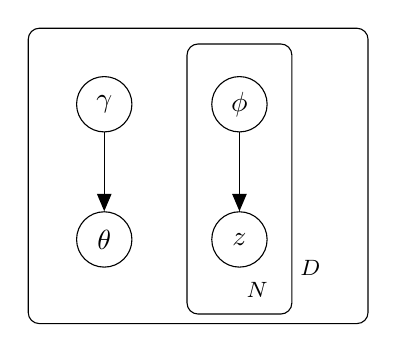
\begin{tikzpicture}
    \node[latent] (y) {$\gamma$};
    \node[latent, below=of y] (t) {$\theta$};
    \node[latent, right=of y] (p) {$\phi$};
    \node[latent, below=of p] (z) {$z$};

    % Edges
    \edge {y} {t};
    \edge {p} {z};
    
    % Plates
    \plate [inner sep=0.3cm, yshift=0.1cm] {pN} {(p)(z)} {$N$};
    {\tikzset{plate caption/.append style={right=0.4cm of #1.south
          east}} \plate [inner sep=0.6cm] {pD} {(y)(t)(p)(z)} {$D$}};
  \end{tikzpicture}
  \caption{\label{fig:lda_vi} Graphical model for the approximate
    posterior for variational inference.}
\end{figure}

To best approximate the true posterior, we frame it as an optimization
problem, minimizing $L$ where:

\begin{multline}
L(\gamma, \phi | \alpha, \beta) = D_{KL}\left[ q(\theta, z | \gamma,
  \phi) || p(\theta, z | \alpha, \beta) \right] \\
- \log p(w | \alpha, \beta)
\end{multline}

This optimization has closed form coordinate descent equations for
LDA, because the Dirichlet is conjugate to the Multinomial
distribution. This computational convenience comes at the expense of
robustness, making it difficult to apply to other more complicated
topic models \cite{blei2003latent}.

\citeauthor{DBLP:journals/corr/abs-1711-05597} provides a good
overview of the state-of-the-art VI techniques
\cite{DBLP:journals/corr/abs-1711-05597}, and we will not attempt to
replicate their work here.

\subsection{Choosing an Inference Method}
\label{sub:choosing-inference}
How do we know which technique to use to approximate the posterior
density? MCMC methods are computationally more intensive, but provide
samples that are approximately exact from the target posterior
density. In contrast, VI methods view the problem as an optimization
problem, which allows it to utilize efficient learning algorithms such
as stochastic optimization. This is much quicker to compute, and is
suited for larger datasets.

There are many different MCMC sampling methods. Gibbs sampling
requires conjugacy of the prior and posterior distributions. When this
is not possible (in DTM for example), VI methods can perform better
than other sampling methods in the MCMC family.

However, a closer look at the different inference approximation
algorithms also shows that the performance differences can be
explained away by setting certain smoothing hyperparameters
\cite{asuncion-2012-smoot-infer}.

\section{Example Topic Model Training}
To see topic modeling in action, we train them on a dataset of
scientific papers. This dataset was obtained from Kaggle, and contains
all papers from the Neural Information Processing Systems (NIPS)
conference from 1987 to 2016, along with the paper
metadata\footnote{\url{https://www.kaggle.com/benhamner/nips-papers}}.
Jupyter notebooks for data exploration and model training can be found
here
\footnote{\url{https://github.com/jethrokuan/data-science-notebooks/tree/master/04\%20-\%20Topic\%20Modeling\%20(UROP)/nips-papers}}.

We trained LDA and DTM, using implementations readily available within
Gensim, a popular topic modeling library.

To clean the raw text, we lemmatize, remove stop words, and keep only
noun phrases. After removing tokens that rarely occur, or occur too often
to be meaningful, the corpus of 7241 documents produced a dictionary
of 54254 unique tokens. We set $K = 30$ topics.

We trained LDA for 200 passes, which took 44 minutes, and the full
results are shown in the appendix (~\autoref{fig:lda_results}).

\begin{figure}[ht]
  \begin{tabularx}{\linewidth}{|r | X|}
    \hline
    1 & mixture, covariance, likelihood, component, density, estimation \\ \hline
    2 & policy, action, reward, game, agent, regret \\ \hline
    3 & theorem, bound, cluster, lemma, complexity, proof \\ \hline
  \end{tabularx}
  \caption{\label{fig:lda_trunc} Short selection of LDA topic results.}
\end{figure}

~\autoref{fig:lda_trunc} shows a selection of the topics generated by
LDA. Each row is a learned abstract topic, and the words are presented
in order of decreasing probability. We see that LDA is able to learn
several meaningful topics: topic 1 is likely to be of high proportion
in documents about topic modeling, and similarly topic 2 in documents
about reinforcement learning, and topic 3 in documents about
algorithmic complexity.

To train DTM, we discretized the corpus into time slices that span a
year. Unlike LDA, DTM was trained until convergence. This renders any
quantitative comparisons ineffective. DTM took 3.9 hours to train. We
inferred the topic distributions for three time slices, and they are
displayed in the appendix (~\autoref{fig:dtm_slice1},
~\autoref{fig:dtm_slice2}, ~\autoref{fig:dtm_slice3}). We also show
the evolution of a single topic across 10 time slices in
~\autoref{fig:dtm_evo}.

\begin{figure}[ht]
  \begin{tabularx}{\linewidth}{|r | X|}
    \hline
    1 & energy, field, temperature, transition, boltzmann, spin \\ \hline
    2 & energy, field, temperature, transition, boltzmann, spin \\ \hline
    3 & field, energy, temperature, transition, boltzmann, \bf{markov}
    \\ \hline
    
  \end{tabularx}
  \caption{\label{fig:dtm_trunc} Evolution of topic 27 over time in
    the trained DTM model. This one indicates ``markov'' is being
    mentioned more in this abstract topic, in later years. }
\end{figure}

By comparing the three time slices, we notice that the highly probable
words in each topic remain largely unchanged across each time slice in
this dataset. ~\autoref{fig:dtm_trunc} shows that in the last time
slice, ``markov'' squeezed into the top 6 words of the abstract topic.
Perhaps this is indicative of an increased usage of Markov related
techniques in the later years.

\section{Evaluating Topic Models}
\label{sec:evaluation}
While analysing the results of our trained models, we used human
judgment to evaluate the quality of the abstract topics generated. In
addition, we judged the quality of the topic by how amenable it is to
human interpretation, which may not be suitable, depending on the
task. This evaluation metric is subjective and not reproducible, and
leaves much to be desired.

The unsupervised nature of topic modeling makes model selection
difficult: there are no gold labels for topics and document topic
proportions. The most common evaluation metric is the probability of
held-out documents given a trained model \cite{wallach2009evaluation},
and we refer you to \citeauthor{wallach2009evaluation} for a full
treatment.

To compare the topic models, We look at evaluations from each of the
seminal papers. For LDA, \citeauthor{blei2003latent} computed the
perplexity of held-out documents to evaluate the topic models.
Perplexity is a commonly used metric in language modeling, and is
equivalent to the inverse of the geometric mean per-word likelihood.
Lower perplexity indicates better generalisation performance
\cite{blei2003latent}. In their experiment,
\citeauthor{blei2003latent} used a corpus of scientific abstracts from
the C. Elegans community (5,255 documents with 28,414 terms) and a
corpus of newswire articles (16,333 documents with 23,075 terms). In
both cases, 10\% of the documents were held out for test purposes.
Comparing LDA with pLSA, LDA achieved lower perplexity scores, and LSI
and pLSA suffered from severe overfitting issues. This was attributed
to the ability of LDA to assign probability to a new document without
additional heuristics \cite{blei2003latent}.

In the seminal paper for CTM, \citeauthor{blei2005correlated} fitted
both CTM and LDA to a smaller collection of articles to models of
varying number of topics. It was shown that the average held-out
probability of documents for CTM was consistently better than LDA, and
CTM supported more topics than LDA. This is because CTM is more
expressive than LDA: LDA will only predict words based on latent
topics suggested by observations, but CTM can also predict words
associated with topics correlated with the conditionally probable
topics \cite{blei2005correlated}.

To evaluate DTM, \citeauthor{blei2006dynamic} selected 250 articles
from each of the 120 years between 1881 and 1999 from the Journal
\textit{Science}. The task of predicting the next year in
\textit{Science} given all the articles from the previous years was
considered. Three models were compared: DTM trained on all documents
from previous years, LDA trained on all documents from previous years,
and LDA trained on documents from a single previous year. DTM was
shown to assign a higher likelihood to next year's articles
\cite{blei2006dynamic}. It was also noted that the predictive power of
each model decreases each year, suggesting that factoring time into
the model is important for the task of trend detection in scientific
documents.

\section{Conclusion}
In this paper, we have discussed the importance of topic modeling, and
the opportunities it presents in the domain of scientific documents.
LDA is widely regarded as the simplest topic model, which operates on
the intuition that a document has few topics, and a topic has few
words. LDA has inspired other topic models, such as CTM and DTM, in no
small part due to its simplicity. LDA makes several statistical
assumptions, and in the context of scientific documents some of these
assumptions are not appropriate. CTM and DTM were introduced in
the context of relaxing some of these assumptions.

To demonstrate what topic models are capable of, we trained LDA and
DTM on the NIPS dataset, and provided the Jupyter notebooks for
reference. We also briefly discussed the difficulties faced in
evaluating topic models, that arise from the unsupervised nature of
the problem. We then summarised the evaluation results for each topic
model from the original papers. We note that the evaluation task
differs across each paper, so no combined comparison can be made.

\section{Future Work}
There are many topic models that are not covered in this survey. For
example, the topic models we have covered train only on document text.
Yet, scientific documents often come with useful metadata. The
author-topic model exploits this metadata \cite{rosen2004author}. We
hope to investigate these models in detail in future work.

In addition, there was no attempt to evaluate the trained topic
models, nor was there an attempt to provide a fair comparison between
the topic models. Producing benchmarks for all aforementioned models
on the same corpus should provide immense value to the research
community.

The topic models we have surveyed are directed graphical models.
Despite the recent discoveries in deep learning, LDA, which is over a
decade old, has not been replaced as the mainstay for topic modeling.
There has been promising development in topic modeling with deep
generative models \cite{hinton2009replicated, larochelle2012neural,
  cao2015novel}. This area of research is still relatively unexplored,
and we believe there is much to explore.

\bibliography{survey}

\onecolumn

\section{Appendix}
\label{sec:appendix}

\begin{figure}[ht]
  \centering
  \begin{tabular}{l | l l l l l l}
    &     word0    &      word1 &          word2 &         word3 & word4 &        word5 \\ \hline
    topic0 & optimization & gradient & convergence & iteration & constraint & descent \\
    topic1 & policy & action & reward & agent & reinforcement & transition \\
    topic2 & target & effect & trial & causal & decision & cue \\
    topic3 & distance & tensor & dimension & similarity & transformation & neighbor \\
    topic4 & game & player & strategy & expert & equilibrium & action \\
    topic5 & rule & question & relation & knowledge & concept & symbol \\
    topic6 & neuron & circuit & cell & connection & activity & synapsis \\
    topic7 & image & object & recognition & vision & pixel & segmentation \\
    topic8 & topic & document & word & dirichlet & lda & latent \\
    topic9 & kernel & component & eigenvalue & covariance & basis & operator \\
    topic10 & bound & loss & theorem & proof & complexity & log \\
    topic11 & layer & architecture & gradient & loss & preprint & unit \\
    topic12 & control & trajectory & movement & motor & feedback & hand \\
    topic13 & field & motion & cell & filter & location & direction \\
    topic14 & sequence & event & transition & gene & interaction & expression \\
    topic15 & query & cost & search & code & worker & communication \\
    topic16 & response & neuron & spike & stimulus & population & activity \\
    topic17 & node & tree & inference & graph & message & factor \\
    topic18 & prediction & regression & arxiv & selection & dataset & datasets \\
    topic19 & block & path & implementation & chip & processor & operation \\
    topic20 & unit & energy & equation & noise & generalization & activation \\
    topic21 & memory & pattern & category & capacity & prototype & item \\
    topic22 & source & speech & signal & domain & recognition & frequency \\
    topic23 & word & language & sentence & context & sequence & translation \\
    topic24 & graph & cluster & edge & item & vertex & clustering \\
    topic25 & group & region & brain & level & map & module \\
    topic26 & rank & sparse & column & norm & sparsity & entry \\
    topic27 & regret & arm & bandit & bound & online & round \\
    topic28 & classification & label & classifier & margin & instance & decision \\
    topic29 & inference & density & log & likelihood & estimate & mixture \\
  \end{tabular}
  \caption{\label{fig:lda_results} Top 6 words of the 30 topic distributions from the LDA model trained on the NIPS papers dataset.}
\end{figure}

\begin{figure}[ht]
  \centering
  \begin{tabular}{l | l l l l l l}
    &     word0    &      word1 &          word2 &         word3 & word4 &        word5 \\ \hline
    topic0 & 	node & 	tree & 	graph & 	message & 	path & 	link \\
    topic1 & 	operator & 	rbf & 	kernel & 	regression & 	spline & product \\
    topic2 & 	capacity & 	bound & 	complexity & 	theorem & 	proof & hypothesis \\
    topic3 & 	image & 	object & 	pixel & 	recognition & 	surface & vision \\
    topic4 & 	projection & 	basis & 	selection & 	product & 	pursuit & 	regression \\
    topic5 & 	map & 	motor & 	target & 	eye & 	brain & 	response \\
    topic6 & 	motion & 	direction & 	velocity & 	field & 	trajectory & 	robot \\
    topic7 & 	component & 	density & 	mixture & 	dimension & 	principle & 	mapping \\
    topic8 & 	transfer & 	expert & 	episode & 	rnn & 	decoder & 	translation \\
    topic9 & 	noise & 	estimate & 	variance & 	estimation & 	likelihood & 	criterion \\
    topic10 & 	rule & 	symbol & 	grammar & 	string & 	generalization & 	population \\
    topic11 & 	curve & 	expression & 	eigenvalue & 	eigenvectors & 	gene & 	patient \\
    topic12 & 	classifier & 	classification & 	pattern & 	decision & 	label & 	tree \\
    topic13 & 	speech & 	recognition & 	signal & 	word & 	speaker & 	phoneme \\
    topic14 & 	region & 	group & 	gamma & 	mixture & 	event & 	component \\
    topic15 & 	code & 	transformation & 	rotation & 	translation & 	digit & 	invariance \\
    topic16 & 	neuron & 	memory & 	circuit & 	chip & 	analog & 	connection \\
    topic17 & 	prediction & 	risk & 	loss & 	predictor & 	minimization & 	hypothesis \\
    topic18 & 	cell & 	neuron & 	response & 	activity & 	pattern & 	stimulus \\
    topic19 & 	validation & 	support & 	plane & 	margin & 	hyperplane & 	cross \\
    topic20 & 	equilibrium & 	strategy & 	game & 	position & 	move & 	board \\
    topic21 & 	distance & 	cluster & 	center & 	prototype & 	neighbor & 	assignment \\
    topic22 & 	phase & 	arm & 	learner & 	online & 	strategy & 	bandit \\
    topic23 & 	equation & 	convergence & 	gradient & 	optimization & 	constraint & 	minimum \\
    topic24 & 	unit & 	layer & 	pattern & 	activation & 	backpropagation & 	architecture \\
    topic25 & 	sequence & 	control & 	controller & 	chain & 	protein & 	plant \\
    topic26 & 	action & 	reinforcement & 	control & 	environment & 	controller & 	goal \\
    topic27 & 	energy & 	field & 	temperature & 	transition & 	boltzmann & 	spin \\
    topic28 & 	user & 	query & 	retrieval & 	document & 	word & 	text \\
    topic29 & 	character & 	word & 	letter & 	role & 	recognition & 	language \\
  \end{tabular}
  \caption{\label{fig:dtm_slice1} Top 6 words of the 30 topic distributions in slice 1 of the DTM model trained on the NIPS papers dataset.}
\end{figure}

\begin{figure}[ht]
  \centering
  \begin{tabular}{l | l l l l l l}
    &     word0    &      word1 &          word2 &         word3 & word4 &        word5 \\ \hline
    topic0 & 	node & 	tree & 	graph & 	message & 	path & 	edge \\
    topic1 & 	operator & 	rbf & 	kernel & 	regression & 	spline & 	product \\
    topic2 & 	capacity & 	bound & 	complexity & 	theorem & 	proof & 	concept \\
    topic3 & 	image & 	object & 	pixel & 	recognition & 	surface & 	vision \\
    topic4 & 	projection & 	basis & 	selection & 	product & 	pursuit & 	regression \\
    topic5 & 	map & 	target & 	motor & 	eye & 	response & 	movement \\
    topic6 & 	motion & 	direction & 	velocity & 	field & 	trajectory & 	robot \\
    topic7 & 	component & 	density & 	mixture & 	dimension & 	principle & 	mapping \\
    topic8 & 	transfer & 	expert & 	episode & 	rnn & 	decoder & 	translation \\
    topic9 & 	noise & 	estimate & 	variance & 	estimation & 	likelihood & 	criterion \\
    topic10 & 	rule & 	symbol & 	grammar & 	string & 	generalization & 	population \\
    topic11 & 	curve & 	expression & 	eigenvalue & 	eigenvectors & 	gene & 	patient \\
    topic12 & 	classifier & 	classification & 	pattern & 	decision & 	label & 	tree \\
    topic13 & 	speech & 	recognition & 	signal & 	word & 	speaker & 	phoneme \\
    topic14 & 	region & 	group & 	gamma & 	mixture & 	event & 	component \\
    topic15 & 	code & 	transformation & 	rotation & 	translation & 	digit & 	invariance \\
    topic16 & 	neuron & 	memory & 	circuit & 	chip & 	analog & 	voltage \\
    topic17 & 	prediction & 	risk & 	loss & 	predictor & 	minimization & 	hypothesis \\
    topic18 & 	cell & 	neuron & 	response & 	activity & 	pattern & 	stimulus \\
    topic19 & 	validation & 	support & 	plane & 	margin & 	hyperplane & 	cross \\
    topic20 & 	equilibrium & 	strategy & 	game & 	position & 	move & 	board \\
    topic21 & 	distance & 	cluster & 	center & 	prototype & 	neighbor & 	measure \\
    topic22 & 	phase & 	arm & 	learner & 	online & 	strategy & 	bandit \\
    topic23 & 	equation & 	convergence & 	gradient & 	optimization & 	constraint & 	descent \\
    topic24 & 	unit & 	layer & 	pattern & 	activation & 	backpropagation & 	architecture \\
    topic25 & 	sequence & 	control & 	controller & 	chain & 	protein & 	plant \\
    topic26 & 	action & 	reinforcement & 	control & 	environment & 	controller & 	goal \\
    topic27 & 	energy & 	field & 	temperature & 	transition & 	boltzmann & 	spin \\
    topic28 & 	user & 	query & 	retrieval & 	document & 	word & 	text \\
    topic29 & 	word & 	character & 	letter & 	recognition & 	role & 	language \\
  \end{tabular}
  \caption{\label{fig:dtm_slice2} Top 6 words of the 30 topic distributions in slice 2 of the DTM model trained on the NIPS papers dataset.}
\end{figure}

\begin{figure}[ht]
  \centering
  \begin{tabular}{l | l l l l l l}
    &     word0    &      word1 &          word2 &         word3 & word4 &        word5 \\ \hline
    topic0 & 	node & 	tree & 	graph & 	path & 	message & 	edge \\
    topic1 & 	operator & 	rbf & 	kernel & 	regression & 	spline & 	product \\
    topic2 & 	bound & 	complexity & 	capacity & 	theorem & 	proof & 	concept \\
    topic3 & 	image & 	object & 	recognition & 	pixel & 	vision & 	surface \\
    topic4 & 	projection & 	basis & 	selection & 	product & 	pursuit & 	regression \\
    topic5 & 	map & 	target & 	eye & 	motor & 	movement & 	response \\
    topic6 & 	motion & 	direction & 	velocity & 	trajectory & 	field & 	robot \\
    topic7 & 	component & 	density & 	mixture & 	dimension & 	principle & 	mapping \\
    topic8 & 	expert & 	transfer & 	episode & 	rnn & 	decoder & 	translation \\
    topic9 & 	noise & 	estimate & 	variance & 	estimation & 	likelihood & 	criterion \\
    topic10 & 	rule & 	symbol & 	grammar & 	string & 	generalization & 	knowledge \\
    topic11 & 	curve & 	expression & 	eigenvalue & 	eigenvectors & 	gene & 	patient \\
    topic12 & 	classifier & 	classification & 	pattern & 	decision & 	label & 	accuracy \\
    topic13 & 	speech & 	recognition & 	signal & 	word & 	speaker & 	phoneme \\
    topic14 & 	region & 	group & 	gamma & 	mixture & 	event & 	component \\
    topic15 & 	code & 	transformation & 	rotation & 	digit & 	translation & 	invariance \\
    topic16 & 	memory & 	neuron & 	circuit & 	chip & 	analog & 	voltage \\
    topic17 & 	prediction & 	risk & 	loss & 	predictor & 	minimization & 	hypothesis \\
    topic18 & 	cell & 	neuron & 	response & 	activity & 	pattern & 	stimulus \\
    topic19 & 	validation & 	support & 	plane & 	margin & 	hyperplane & 	cross \\
    topic20 & 	equilibrium & 	strategy & 	game & 	position & 	move & 	board \\
    topic21 & 	distance & 	cluster & 	center & 	prototype & 	neighbor & 	measure \\
    topic22 & 	phase & 	arm & 	learner & 	online & 	strategy & 	bandit \\
    topic23 & 	equation & 	convergence & 	gradient & 	optimization & 	constraint & 	descent \\
    topic24 & 	unit & 	layer & 	pattern & 	architecture & 	backpropagation & 	activation \\
    topic25 & 	control & 	sequence & 	controller & 	chain & 	protein & 	plant \\
    topic26 & 	action & 	reinforcement & 	control & 	environment & 	controller & 	goal \\
    topic27 & 	field & 	energy & 	temperature & 	transition & 	boltzmann & 	markov \\
    topic28 & 	query & 	user & 	retrieval & 	document & word & text \\
    topic29 & word & character & letter & recognition & language & role \\
  \end{tabular}
  \caption{\label{fig:dtm_slice3} Top 6 words of the 30 topic distributions in slice 3 of the DTM model trained on the NIPS papers dataset.}
\end{figure}

\begin{figure}[ht]
  \centering
  \begin{tabular}{|l | l |}
    \hline
     time slice & words \\ \hline
    0 & node, tree, graph, message, path, link, edge, cycle, branch, parent \\ \hline
    1 &	node, tree, graph, message, path, edge, link, cycle, branch, parent \\ \hline
    2 &	node, tree, graph, path, message, edge, link, cycle, branch, parent \\ \hline
    3 & node, tree, graph, path, message, edge, link, cycle, parent, branch \\ \hline
    4 &	node, tree, graph, path, edge, message, link, parent, cycle, level \\ \hline
    5 &	node, tree, graph, path, edge, message, link, parent, level, leaf \\ \hline
    6 &	node, tree, graph, path, edge, message, link, parent, leaf, level \\ \hline
    7 &	node, tree, graph, path, edge, message, link, parent, leaf, propagation \\ \hline
    8 &	node, tree, graph, path, edge, message, parent, propagation, belief, link \\ \hline
    9 &	node, tree,	graph, path, edge, belief, message, propagation, parent,	leaf \\ \hline
  \end{tabular}
  \caption{\label{fig:dtm_evo} Evolution of Topic 1 across 10 time
    slices in the DTM model trained on the NIPS papers dataset.}
\end{figure}

\end{document}
